\section{Conclusion and Discussion}

\subsection{ODE model}
The fitting method still needs improvement. For the fitting iterations, we only involve infectious data in residual function and minimize the error in fitting the infectious data to get an initial beta. Then we use the beta for following iterations for minimizing the error in fitting the death data and then the hospitalized data and then the recovery data. The beta doesn't change much during the iterations. For example, for the after vaccine outbreak, the beta after each iteration is : 0.18322830 -> 0.14602370 ->  0.20936286 -> 0.26362917. Though the beta doesn't change much during these iterations, every iteration fits the assigned curve well but doesn't perform as well in other curves (see Figure \ref{sir5}). So it is still not scientific enough to fit for only one parameter and one curve for one iteration. It would be better if all the curves are fitted at the same time in every iteration.
\begin{figure}
	\centering
	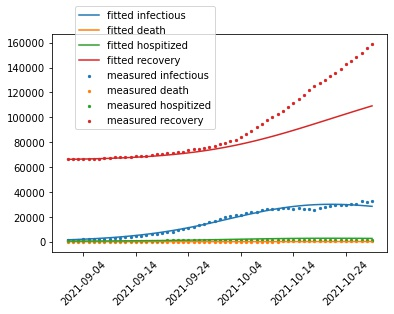
\includegraphics[scale = 0.5]{Final/ode model/after fit all-2.jpg}
	\caption{Fitting Results of the Second Outbreak}
	\label{sir5}
\end{figure}

Another point for improvement is to find a scientific way to measure and estimate the number of susceptible cases in real life spread. We get a good fit result by manually assigning the number of initial susceptible cases and we also see other researchers who set the number of initial susceptible cases as a value suggested by domain experts. So it would be very helpful for using the SIR and SEIR ODE model to research on real life problems if there is a more systematic and scientific method to get the number of S state cases in real life.

\subsection{Agent-based model}
The results of the agent-based model reveal the importance of vaccination and strict mask policies. Even the delta variant is highly infectious, with vaccination and strict mask policies the number of infections is still able to be controlled small. The mobility takes an important role when mask policies are relatively loose but contributes little to the spread of COVID-19 when mask policies are strict. Therefore, we strongly suggest that high vaccination rate and strict mask policies are vital for fighting against COVID-19.

However, there are several aspects that may be improved in the future research.

First, we assume that lots of parameters are constant within out model, such as test probability, contact tracing probability, quarantine period, etc. However, these parameters changes during the pandemic and highly depends on the government policies and the pandemic situation. Future research can focus on how the model the change of these parameters so that the model can represent the reality better.

What's more, covasim calculates the waning effect of vaccines based on the decreasing of neutralizing antibody \cite{khoury2021level} and calculates the effectiveness against the delta variant based on this paper \cite{mlcochova2021sars}. Because of limited time and knowledge, we are not able to verify the correctness of these values and models. The waning effect of vaccines and the effectiveness against different variants are hot topics in this area. We should also notice that Singapore has started the vaccine booster program from October 1st while the impact of the booster is still under research. Therefore, future research may be able to model the effectiveness of vaccines in a more accurate way.